\chapter{Introduzione}
\raggedright{\section{Descrizione richiesta del progetto}}

È richiesto di migliorare e potenziare un sistema informativo già esistente per la gestione di bibliografie. Il sistema deve essere capace di salvare e organizzare i riferimenti bibliografici degli utenti.  In particolare, è possibile inserire, modificare, rimuovere riferimenti bibliografici di diverso tipo (e.g.: articoli scientifici su conferenza o rivista, libri, risorse on-line, dataset, etc.).
Ciascun riferimento è caratterizzato da un titolo univoco, un elenco di autori, una data, un URL (obbligatorio solo per risorse on-line), un DOI (facoltativo, ma univoco ove presente), e una descrizione testuale in cui l’utente può indicare aspetti significativi.
Inoltre, un riferimento può essere associato a un insieme di rimandi, ovvero di altri riferimenti presenti nel sistema che vengono menzionati nel testo.

Un utente, infine, può definire un insieme di categorie personalizzate e possibilmente gerarchiche, e associare ciascun riferimento a una o più categorie. Per organizzazione gerarchica delle categorie si intende la possibilità di specificare che una certa categoria (e.g.: “Informatica”) ha una o più sottocategorie (e.g.: “Basi di Dati” o “Testing”).

Non è possibile introdurre dipendenze cicliche, ovvero non è possibile che una categoria sia una sottocategoria (anche transitivamente) di sé stessa. L’appartenenza a una sottocategoria implica l’appartenenza a tutte le sue super-categorie. Non è pertanto possibile associare esplicitamente a un riferimento una categoria e una sua super-categoria.

Il sistema permette infine di effettuare interrogazioni avanzate, con possibilità di filtraggio per una o più categorie, per data, per parole chiave e per autore. Inoltre, è possibile ordinare i riferimenti per numero di citazioni ricevute, ovvero per il numero di volte in cui il riferimento è presente nei rimandi di altri riferimenti.

Inoltre è richiesto lo sviluppo di nuove funzionalità da integrare nel sistema informativo già esistente.

\raggedright{\section{Stato progetto originale}}
L'applicativo originale, seppur lasciato in ottimo stato, presenta alcuni punti deboli per quanto riguarda la progettazione software e usabilità. In particolare, verranno mostrati le varie funzionalità e i vari aspetti dell'applicativo che verranno modificati affinché possa rispettare gli standard odierni.
\raggedright{{\subsection{Basi di dati}}}
         \begin{center}
     \hspace{-1cm}
            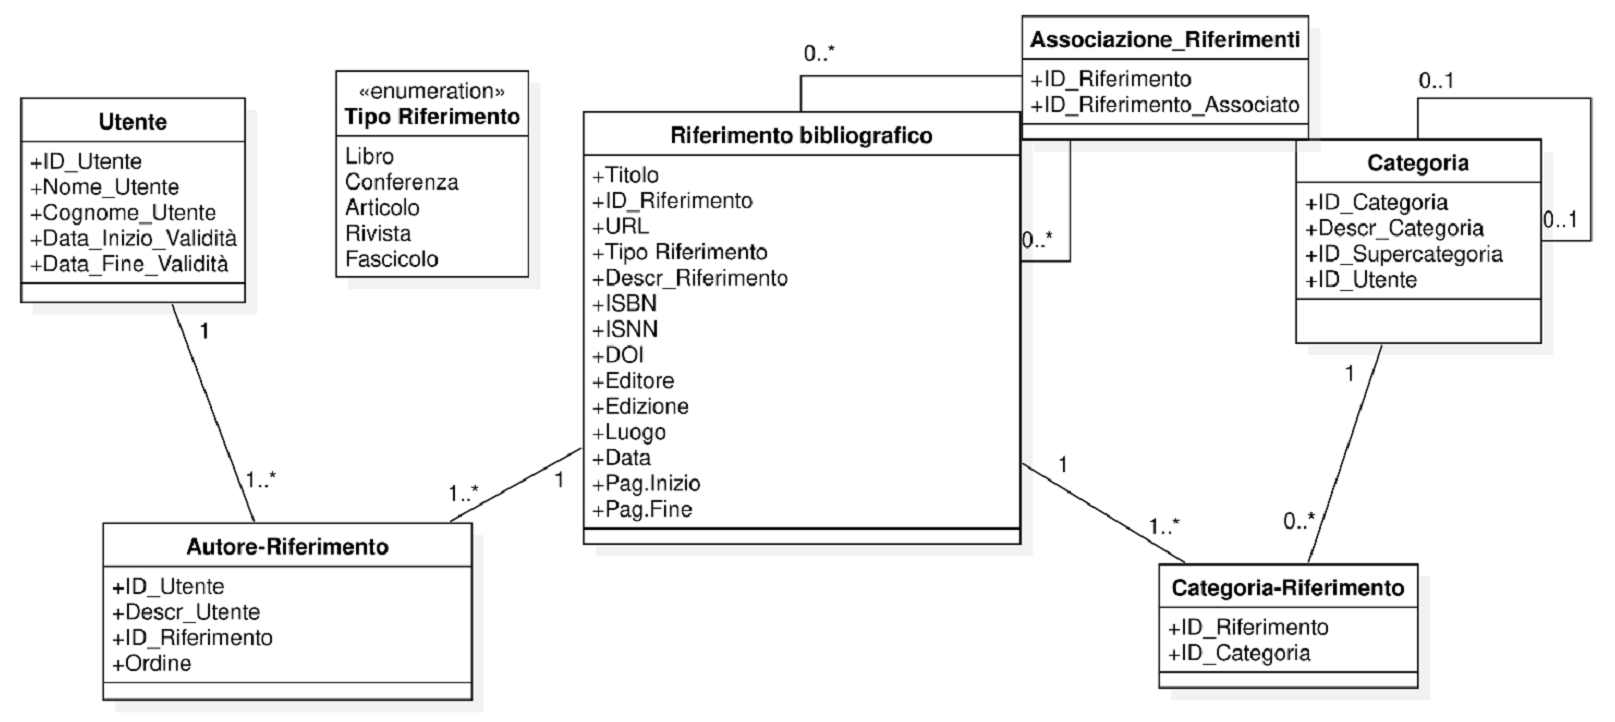
\includegraphics[width=.90\textwidth]{Immagini/VecchioProgetto/UML Basi di Dati pre ristrutturato.png} 
        \end{center}
La Basi di Dati originale è stata implementata nel modo seguente: \\la tabella \textit{Utente} descrive il possible utente che accede alla piattaforma dei riferimenti bibliografici. Contiene un identificativo univoco, un nome e cognome e due date di inzio e fine validità rispettivamente. \\
La tabella \textit{Autore-Riferimento} descrive il possible ideatore o relatore in base a che tipologia di riferimento bibliografico si analizzi. \\
La tabella \textit{Riferimento Bibliografico} descrive il possible riferimento bibliografico e le sue caratteristiche in base alla tipologia. \\
La tabella \textit{Categoria} descrive una categoria e le sue possibili sottocategorie. \\
La tabella \textit{Associazione-Riferimenti} è un descrittore di un riferimento che può essere associato a un insieme di rimandi. \\
La tabella \textit{Categoria-Riferimento} è un descrittore di una categoria che è associata ad  un riferimento. \\
\raggedright{\subsection{Applicativo Java}}
L’approccio di design utilizzato è quello di un sistema Object Oriented sviluppato in Java che dipende strettamente da un database PostgreSQL. L’ambiente di sistema è un qualsiasi sistema operativo non-mobile (quindi desktop) fornito di una connessione al database.
\begin{center}
    \hspace{-1cm}
        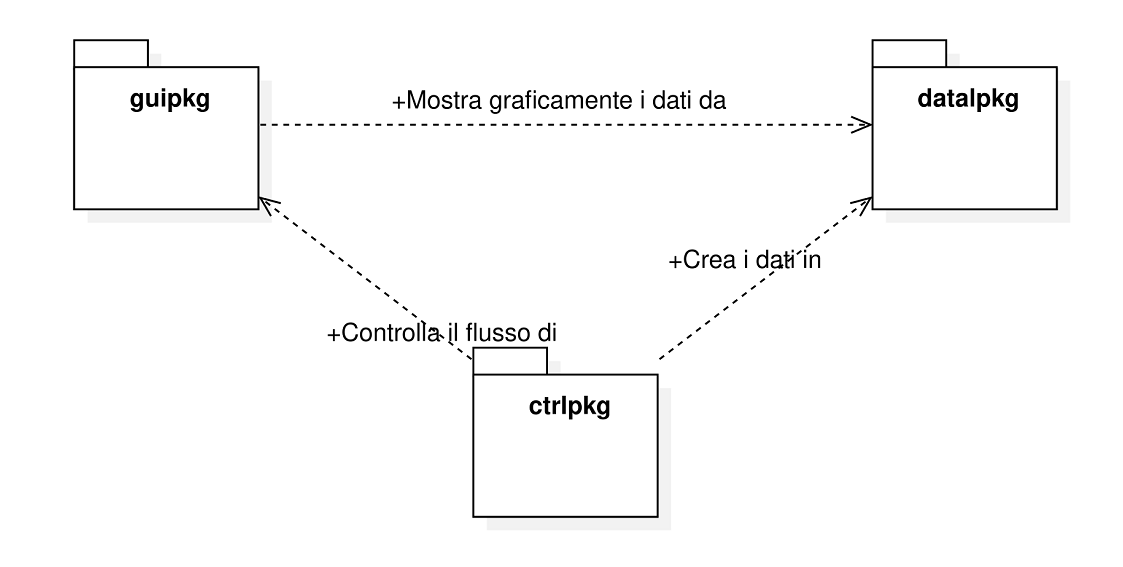
\includegraphics[width=.90\textwidth]{Immagini/VecchioProgetto/UML OO Java vecchioProgetto.png} 
\end{center}

Il sistema è costituito da 3 elementi principali, rappresentati in package: \\
\textit{guipkg}, per la definizione delle interfacce grafiche e le loro interazioni; \\ 
\textit{datalpkg}, per la definizione delle classi di dati che andranno trattati e mostrati;\\
\textit{ctrlpkg}, per la definizione dei collegamenti e delle varie interazioni tra sistema e database esterno.

\raggedright{\section{Migliorie del progetto originale e nuove funzionalità}}
La nuova versione del progetto prevede la modifica delle seguenti funzionalità:
\begin{itemize}
    \item \label{nuovo:accesso} Nuovo sistema di accesso: il sistema non prevederà l'utilizzo dell'ID utente ma di una email e password apposita. Durante la registrazione verrà richiesto infatti di inserire le due informaizoni che saranno poi salvate nel database. Inoltre, per preservare la sicurezza degli utenti, le password verranno criptate.
    \item Rimozione visibilità di ID accesso durante la registrazione: poiché l'utente non può più sapere il suo identificativo, non verrà mostrato il suo ID durante la registrazione.
    \item Potenziamento modalità di ricerca: la ricerca di riferimenti, citazioni e categorie verrà modificato e sarà più intuitivo ed efficiente.
    \item Apertura collegamenti: l'applicativo sarà capace di aprire gli URL inseriti per migliorare l'esperienza dell'utente, funzionalità mancante dell'applicativo originale.
    \item Impostazioni utente: verrà aggiunta la possibilità di modificare le proprie credenziali mediante un menù apposito.
    \item Miglioramento dell'interfaccia grafica: la GUI sarà totalmente ridisegnata per rispettare criteri di buona usabilità e con lo scopo di migliorare l'affordance iniziale, in tal modo da poter soddisfare più utenti possibili e di coprire tutte le possibili esigenze.
\end{itemize}
